\documentclass[conference]{IEEEtran}
\usepackage{tikz}
\usetikzlibrary{positioning, shapes.geometric, arrows.meta, fit, calc,
                 backgrounds, shadows.blur}
\usepackage[T1]{fontenc}

\begin{document}

\begin{figure}[!t]
\centering
\resizebox{\columnwidth}{!}{%
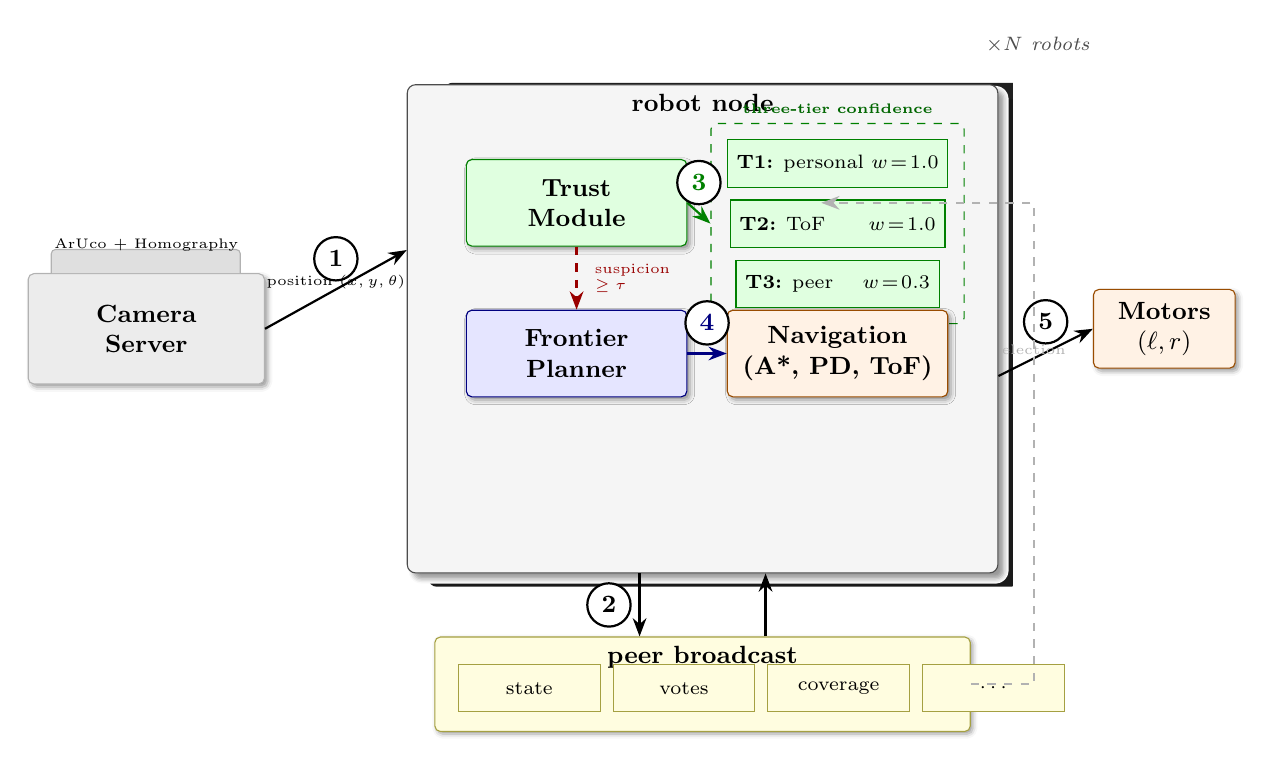
\begin{tikzpicture}[
    >=Stealth,
    % Colours
    trustfill/.style  ={fill=green!12},
    trustdraw/.style  ={draw=green!50!black},
    planfill/.style   ={fill=blue!10},
    plandraw/.style   ={draw=blue!50!black},
    navfill/.style    ={fill=orange!10},
    navdraw/.style    ={draw=orange!60!black},
    peerfill/.style   ={fill=yellow!12},
    peerdraw/.style   ={draw=yellow!60!black},
    camfill/.style    ={fill=gray!15},
    camdraw/.style    ={draw=gray!60},
    % Module box
    module/.style={
        draw, rectangle, rounded corners=2pt,
        minimum width=26mm, minimum height=11mm,
        align=center, font=\small\bfseries,
        blur shadow={shadow blur steps=3, shadow xshift=0.4mm,
                     shadow yshift=-0.4mm}
    },
    % Inner cell (like state machine entries)
    cell/.style={
        draw, rectangle, minimum width=18mm, minimum height=6mm,
        align=center, font=\scriptsize, fill=white
    },
    % Numbered circled labels
    circnum/.style={
        circle, draw=black, fill=white, inner sep=0pt,
        minimum size=5.5mm, font=\small\bfseries
    },
    % Arrows
    arrow/.style={-Stealth, thick},
    darrow/.style={Stealth-Stealth, thick},
    dasharrow/.style={-Stealth, thick, dashed},
]

% ============================================================
%  Camera Server (external — like "client" in Raft diagram)
% ============================================================
\node[module, camfill, camdraw, minimum width=30mm, minimum height=14mm]
    (camera) {Camera\\Server};

% Stylistic "lens" shape on top
\draw[camdraw, fill=gray!25, rounded corners=1.5pt]
    ($(camera.north west)+(3mm,0)$) -- ++(0,3mm) -- ++(24mm,0)
    -- ++(0,-3mm);
\node[font=\tiny, above=1.5mm of camera] {ArUco + Homography};

% ============================================================
%  Robot Node (main box — like "server" in Raft)
%  Stacked appearance: two shadow copies behind
% ============================================================

% Shadow copies (N=5 robots)
\begin{scope}[on background layer]
    \fill[gray!25, rounded corners=3pt]
        ($(camera.east)+(22mm,-30mm)$) rectangle ++(75mm,62mm);
    \fill[gray!20, rounded corners=3pt]
        ($(camera.east)+(20mm,-32mm)$) rectangle ++(75mm,62mm);
\end{scope}

% Main robot node container
\node[draw=black!70, rectangle, rounded corners=3pt,
      fill=gray!8, minimum width=75mm, minimum height=62mm,
      blur shadow={shadow blur steps=4},
      right=18mm of camera, yshift=0mm]
    (robot) {};
\node[font=\small\bfseries, anchor=north] at (robot.north) {robot node};

% ---- Trust Module ----
\node[module, trustfill, trustdraw, minimum width=28mm]
    (trust) at ($(robot.center)+(-16mm, 16mm)$)
    {Trust\\Module};

% Trust tiers (like state machine entries x:3, y:9, z:0)
\node[cell, trustfill, trustdraw, right=5mm of trust, yshift=5mm]
    (t1) {\textbf{T1:} personal $w\!=\!1.0$};
\node[cell, trustfill, trustdraw, below=1.5mm of t1]
    (t2) {\textbf{T2:} ToF \quad\; $w\!=\!1.0$};
\node[cell, trustfill, trustdraw, below=1.5mm of t2]
    (t3) {\textbf{T3:} peer \quad $w\!=\!0.3$};

% Group the tiers
\node[draw=green!50!black, rounded corners=2pt, dashed,
      fit=(t1)(t3), inner sep=2mm, label={[font=\tiny\bfseries,
      green!40!black]above:three-tier confidence}] (tiers) {};

% ---- Task Planner ----
\node[module, planfill, plandraw, minimum width=28mm,
      below=8mm of trust]
    (planner) {Frontier\\Planner};

% ---- Navigation ----
\node[module, navfill, navdraw, minimum width=28mm,
      right=5mm of planner]
    (nav) {Navigation\\(A*, PD, ToF)};

% ============================================================
%  Peer Communication (like "log" in Raft — below robot box)
% ============================================================
\node[draw=yellow!60!black, rectangle, rounded corners=2pt,
      peerfill, minimum width=68mm, minimum height=12mm,
      below=8mm of robot, blur shadow={shadow blur steps=3,
      shadow xshift=0.3mm, shadow yshift=-0.3mm}]
    (peer) {};
\node[font=\small\bfseries, anchor=north] at (peer.north)
    {peer broadcast};

% Log-like entries
\node[cell, peerfill, peerdraw] (e1) at ($(peer.center)+(-22mm,-0.5mm)$)
    {state};
\node[cell, peerfill, peerdraw, right=1.5mm of e1]
    (e2) {votes};
\node[cell, peerfill, peerdraw, right=1.5mm of e2]
    (e3) {coverage};
\node[cell, peerfill, peerdraw, right=1.5mm of e3]
    (e4) {$\cdots$};

% ============================================================
%  Numbered flow arrows
% ============================================================

% 1: Camera → Robot (position)
\draw[arrow] (camera.east) -- ($(robot.west)+(0,10mm)$)
    node[circnum, above=1mm, midway] {1};
\node[font=\tiny, below=0mm] at ($(camera.east)!0.5!(robot.west)+(0,8mm)$)
    {position $(x,y,\theta)$};

% 2: Robot ↔ Peer broadcast (bidirectional)
\draw[arrow] ($(robot.south)+(-8mm,0)$) -- ($(peer.north)+(-8mm,0)$)
    node[circnum, left=1mm, midway] {2};
\draw[arrow] ($(peer.north)+(8mm,0)$) -- ($(robot.south)+(8mm,0)$);

% 3: Trust module verifies (internal)
\draw[arrow, green!50!black] (trust.east) -- (tiers.west)
    node[circnum, above=1mm, midway] {3};

% 4: Planner → Navigation (internal)
\draw[arrow, blue!50!black] (planner.east) -- (nav.west)
    node[circnum, above=1mm, midway] {4};

% 5: Robot → Motors (output)
\node[module, navfill, navdraw, minimum width=18mm, minimum height=10mm,
      right=12mm of robot]
    (motors) {Motors\\$(\ell, r)$};
\draw[arrow] ($(robot.east)+(0,-6mm)$) -- (motors.west)
    node[circnum, above=1mm, midway] {5};

% Trust → Planner (internal, dashed — suspicion triggers reassignment)
\draw[dasharrow, red!60!black] (trust.south) -- (planner.north)
    node[font=\tiny, right=1mm, midway, align=left, red!60!black]
    {suspicion\\$\geq\tau$};

% ============================================================
%  Annotations
% ============================================================

% "N = 5 robots" label on stacked shadows
\node[font=\scriptsize\itshape, gray!60!black]
    at ($(robot.north east)+(5mm,5mm)$) {$\times N$ robots};

% Election arrow from peer back to trust
\draw[dasharrow, gray!60] ($(peer.east)+(0,0)$) -| ++(8mm,20mm)
    |- ($(trust.east)+(17mm,0)$)
    node[font=\tiny, above, pos=0.25] {election};

\end{tikzpicture}%
}
\caption{REIP robot node architecture. \textcircled{\small 1}~Camera server
sends ArUco-derived pose. \textcircled{\small 2}~Peer state is broadcast and
received via UDP. \textcircled{\small 3}~Three-tier trust module verifies
leader commands before execution. \textcircled{\small 4}~Frontier planner
feeds A*-routed waypoints to the PD navigation controller.
\textcircled{\small 5}~Motor commands are issued. If suspicion exceeds
threshold~$\tau$, the trust module triggers impeachment and re-election
(dashed red).}
\label{fig:reip_node}
\end{figure}

\end{document}
